\documentclass[a4paper,10pt]{article}
\usepackage[margin=0pt]{geometry}
\usepackage{fontspec}
\setmainfont{texgyreheros-regular.otf}[BoldFont=texgyreheros-bold.otf,ItalicFont=texgyreheros-italic.otf,BoldItalicFont=texgyreheros-bolditalic.otf]
\usepackage{tikz}
\usepackage{enumitem}
\usepackage[colorlinks=true,urlcolor=blue]{hyperref}
\definecolor{canvas}{HTML}{F2F2F7}
\definecolor{muted}{HTML}{8A8A8E}
\definecolor{chip}{HTML}{EEEEEE}
\definecolor{rulegray}{HTML}{DADADD}
\pagestyle{empty}
\setlength{\parindent}{0pt}
\setlist[itemize]{leftmargin=3.2mm,labelsep=1.5mm,itemsep=1pt,topsep=2pt,parsep=0pt,label=\textbullet}
\newcommand{\tagpill}[1]{\tikz[baseline=(tag.base)]\node[fill=chip,rounded corners=1.3mm,inner xsep=2mm,inner ysep=.5mm,font=\fontsize{8}{9}\selectfont](tag){#1};\hspace{.5mm}}
\newcommand{\remote}{\hfill\tikz[baseline=(r.base)]\node[fill=chip,rounded corners=1mm,text=muted,inner xsep=2mm,inner ysep=.5mm,font=\fontsize{6.5}{7}\selectfont](r){REMOTE};}
\newcommand{\sectionlabel}[2]{
 \node[anchor=west,text=muted,font=\bfseries\fontsize{7.5}{9}\selectfont,inner sep=0pt] (s) at (8,-#1) {#2};
 \draw[rulegray,line width=.35pt] ([xshift=3mm]s.east) -- (202,-#1);
}
% Card coordinates and dimensions are in millimetres from the top-left corner.
\newcommand{\card}[3]{
 \fill[white,rounded corners=2.5mm] (8,-#1) rectangle (202,{-#1-#2});
 \node[anchor=north west,inner sep=0pt] at (14,{-#1-4}) {\begin{minipage}{182mm}\fontsize{8.5}{10}\selectfont\raggedright #3\end{minipage}};
}
\newcommand{\job}[3]{\textbf{#1}\remote\\\textbf{#2}\\{\color{black!65}#3}\par}
\newcommand{\stack}[1]{\vspace{2pt}\textbf{Tech stack:} #1\par}
\newcommand{\website}[1]{\vspace{2pt}\href{https://#1}{\underline{#1}}}
\begin{document}
\null
\begin{tikzpicture}[remember picture,overlay,x=1mm,y=1mm]
\begin{scope}[shift={(current page.north west)}]
 \fill[canvas] (0,0) rectangle (210,-297);
 \fill[white] (0,0) rectangle (210,-27);
 \node[anchor=north west,inner sep=0pt] at (8,-7) {\begin{minipage}{90mm}
 {\fontsize{15}{17}\selectfont\textbf{Gleb Ambrazhevich}}\\[-1pt]
 {\fontsize{10}{12}\selectfont\textbf{Senior Frontend Engineer}}\\
 {\fontsize{9}{11}\selectfont\color{muted}+381 63-773-59-75}
 \end{minipage}};
 \node[anchor=north east,inner sep=0pt,align=right,font=\fontsize{8.5}{11}\selectfont] at (202,-7) {
 \textbf{Belgrade, Serbia}\\
 \href{mailto:glebikx@gmail.com}{\textcolor{black}{glebikx@gmail.com}}\\
 \href{https://linkedin.com/in/gleb-ambrazhevich-27ab66190/}{\underline{linkedin.com/in/gleb-ambrazhevich-27ab66190/}}};
 \sectionlabel{32}{ABOUT ME}
 \card{37}{20}{Senior Frontend Engineer with 7 years of experience building analytics-heavy dashboards, marketing platforms, eCommerce and IoT products. I combine frontend architecture with a deep understanding of browser rendering, scheduling and performance. My focus: scalable interfaces, experimentation tools and AI-agent workflows where correctness matters.}
 \card{61}{43}{
 \job{Senior Frontend Engineer at Apliteni}{Jan 2024 - Present}{Tallinn, Harjumaa, Estonia}
 \begin{itemize}
 \item Built \textbf{UI virtualization} with pseudonodes: native Ctrl+F and stable scrolling across \textbf{100k+ rows}, within browser DOM and memory limits.
 \item Moved landing pages to \textbf{Framer}, letting designers launch campaigns without engineering support.
 \item Built an \textbf{AI-agent CV screening workflow} to improve recruiter productivity and shortlist relevance.
 \end{itemize}
 \stack{React, Nest.js, TypeScript, Redux, TanStack Query, Zustand, Playwright, Tailwind, Vite, GitLab CI/CD, Sentry, Docker, REST API}
 \website{apliteni.com}
 }
 \card{108}{43}{
 \job{Senior Frontend Engineer at Dimension Four}{May 2022 - Dec 2023}{Skien, Vestfold og Telemark, Norway}
 \begin{itemize}
 \item \textbf{Architected a headless IoT frontend} from scratch: a data-transformation layer and embeddable widgets on a unified GraphQL API, including live public statistics for municipalities.
 \item Built a \textbf{live operator dashboard} with alerts, tables and graphs using GraphQL subscriptions.
 \item Created a \textbf{framework-agnostic Lit library} of charts, counters and maps for React, Angular and plain websites.
 \end{itemize}
 \stack{React, TypeScript, Apollo Client, Lit, Jest, Material UI, Webpack, Sentry, GraphQL API}
 \website{dimensionfour.io}
 }
 \card{155}{43}{
 \job{Frontend Engineer at Apple (Contract via NVP Software)}{Apr 2021 - Apr 2022}{Belmont, California, United States}
 \begin{itemize}
 \item Developed \textbf{configurable campaign templates} for regional and client needs, accelerating launches and onboarding without custom code.
 \item Used \textbf{RxJS asynchronous flows} in live previews to eliminate race conditions and stale fields.
 \item Built \textbf{dynamic campaign forms} with validation, dependencies, user rights, localization and approval flows from draft to submission.
 \end{itemize}
 \stack{React, JavaScript, Redux, RxJS, Ramda.js, Jest, Storybook, Ant Design, Webpack, REST API}
 \website{partnerhub.apple.com}
 }
 \card{202}{18}{
 \textbf{Frontend Developer at Facepass}\\
 \textbf{Feb 2019 - Mar 2021}\par
 \stack{React, Next.js, TypeScript, Redux, Storybook, SCSS-Modules, Webpack}
 }
 \sectionlabel{226}{SKILLS}
 \card{231}{34}{
 \tagpill{React.js}\tagpill{Next.js}\tagpill{TypeScript}\tagpill{TanStack Query}\tagpill{Zustand}\tagpill{RxJS}\tagpill{Apollo Client}\tagpill{Redux}\par\vspace{2pt}
 \tagpill{Frontend Architecture}\tagpill{Design Systems}\tagpill{Performance Optimization}\tagpill{SSR/CSR}\tagpill{Accessibility}\par\vspace{2pt}
 \tagpill{Jest}\tagpill{React Testing Library}\tagpill{Playwright}\par\vspace{2pt}
 \tagpill{Storybook}\tagpill{Tailwind CSS}\tagpill{Styled-Components}\tagpill{Shadcn}\tagpill{SCSS}\par\vspace{2pt}
 \tagpill{REST API}\tagpill{GraphQL}\tagpill{WebSockets}\par\vspace{2pt}
 \tagpill{Monorepo}\tagpill{CI/CD}\tagpill{Git}\tagpill{Vite}\tagpill{Webpack}
 }
 \sectionlabel{271}{EDUCATION}
 \card{276}{16}{\textbf{Bachelor of Marketing}\\\textbf{2013 - 2018}\\{\color{black!65}Belarusian State Technological University}}
\end{scope}
\end{tikzpicture}
\end{document}
